\documentclass{article}
\usepackage{style}
\begin{document}
\maketitle
\tableofcontents
\section{Introducción}
El algoritmo genético enfatiza la importancia de la cruza y la mutación, al igual que la selección probabilistica.
En esta práctica se implementó el algoritmo genético más simple:
\begin{itemize}
	\item Generar aleatoriamente una población inicial.
	\item Calcular la aptitud de cada individuo.
	\item Seleccionar probabilisticamente con base en la aptitud.
	\item Aplicar cruza y mutación para generar la siguiente población.
	\item Ciclar hasta que las condiciones finales se cumplan.
\end{itemize}
Esta técnica fue propuesta por DeJong [137], y ha sido el método más comúnmente
usado desde los orígenes de los algoritmos genéticos. El algoritmo es simple, pero
ineficiente (su complejidad es O(n 2 ). Asimismo, presenta el problema de que el
individuo menos apto puede ser seleccionado más de una vez.
\section{Contenido}
\subsection{Algoritmo con 5 generaciones}
\begin{figure}[h!]
	\centering
	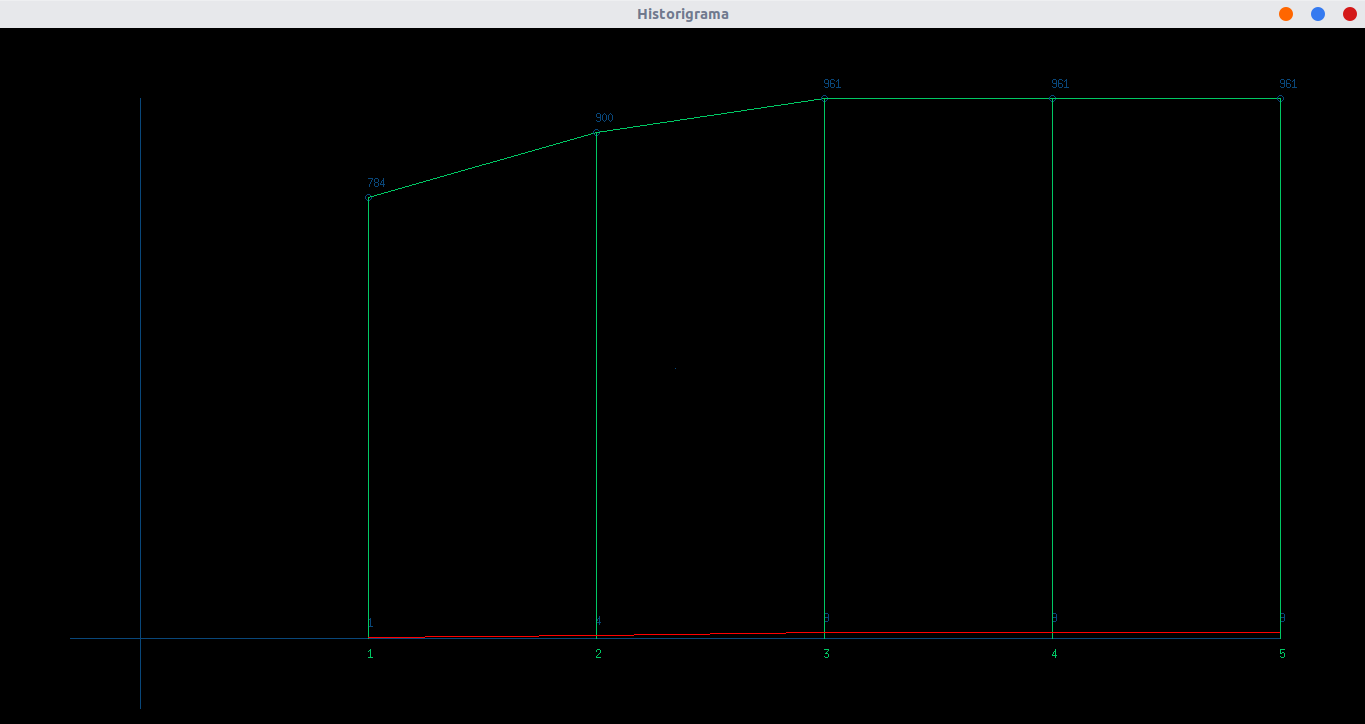
\includegraphics[scale=.3]{5gen}
\end{figure}
\newpage
\subsection{Algoritmo con 10 generaciones}
\begin{figure}[h!]
	\centering
	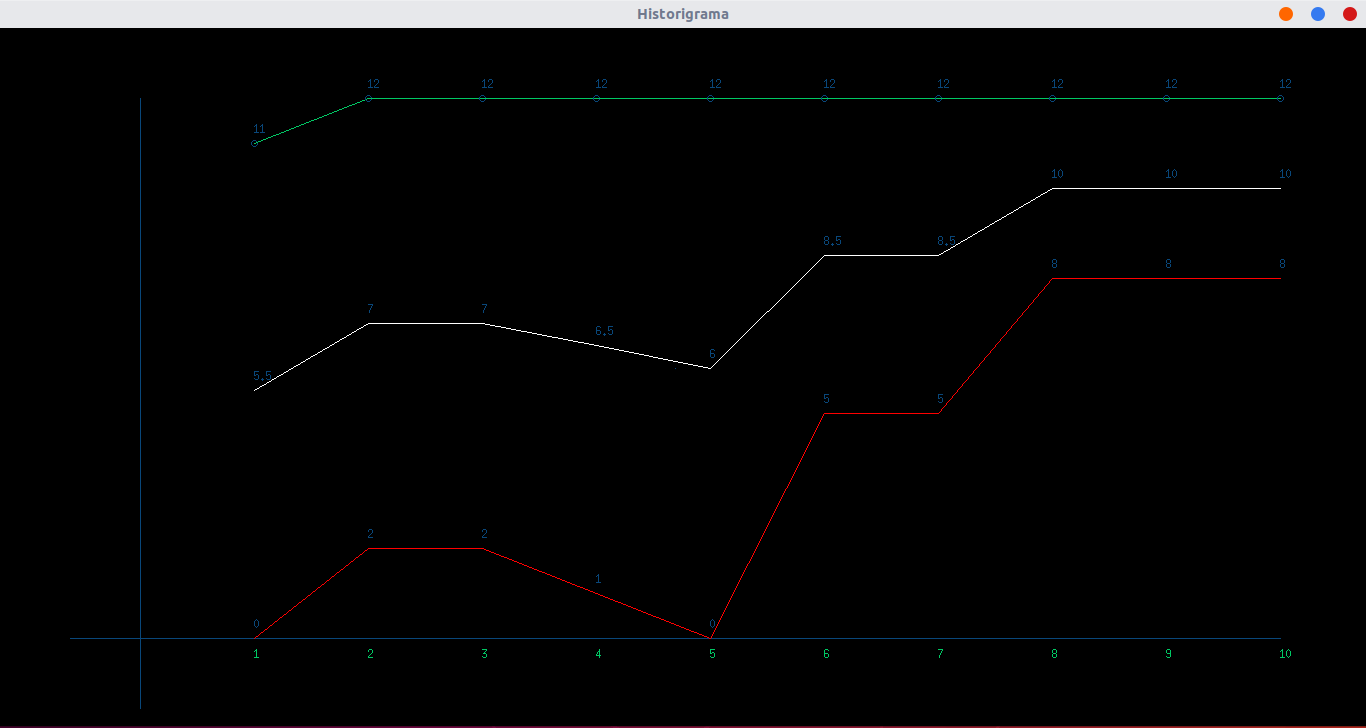
\includegraphics[scale=.3]{10gen}
\end{figure}
\subsection{Algoritmo con 15 generaciones}
\begin{figure}[h!]
	\centering
	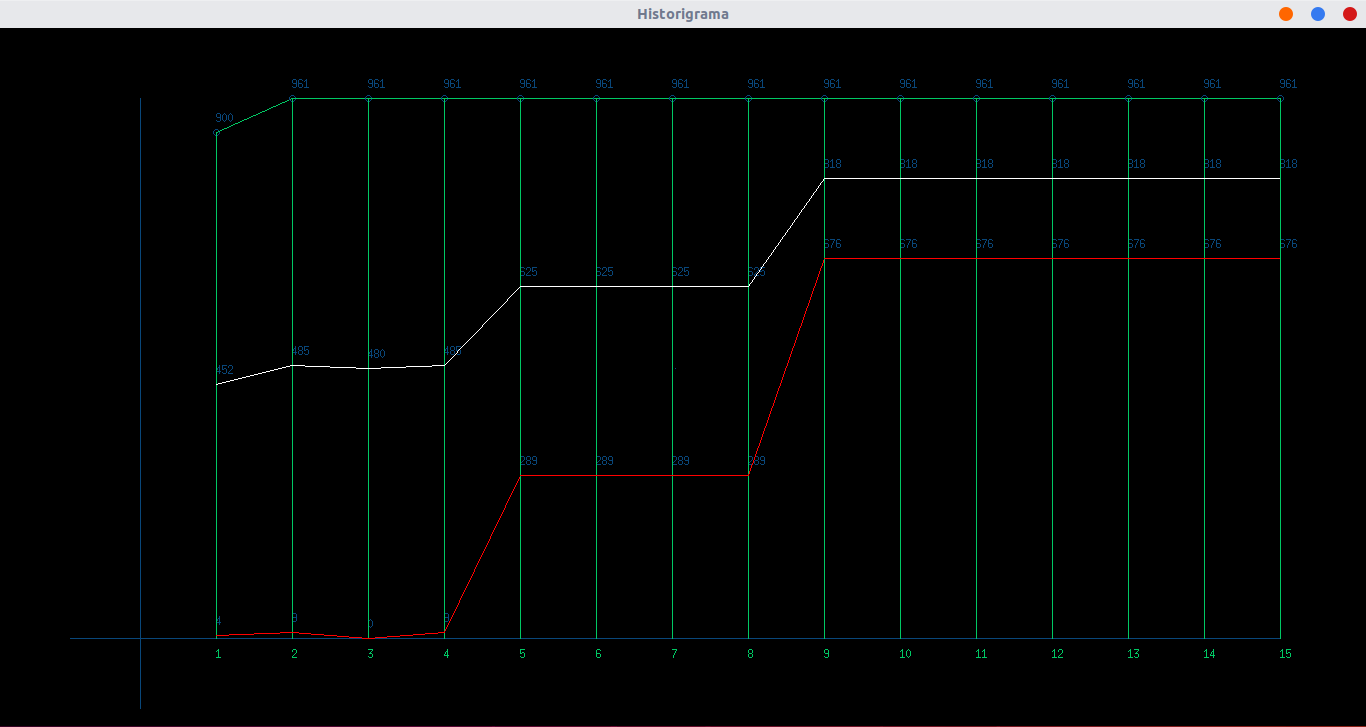
\includegraphics[scale=.3]{15gen}
\end{figure}
\section{Conclusión}
Este algoritmo es el algoritmo genético más simple, pero el más popular.
\end{document}